\subsection{Performance}

\autoref{figure:time-jit-interpreter} shows that the interpreter has far better performance than the JIT for short tests. As the test duration increases the JIT increases in performance, eventually stabilising at approximately 2x faster execution time than the interpreter.

\begin{figure}
    \centering
    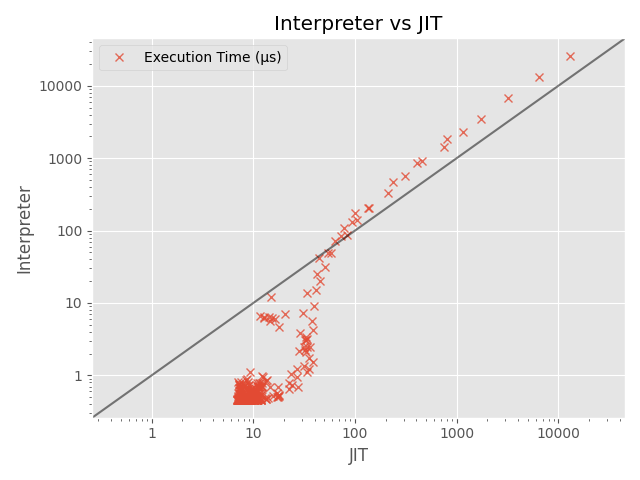
\includegraphics{output/graphs/scatter/time.png}
    \caption{Execution time of all tests for the JIT against the interpreter.}
    \label{figure:time-jit-interpreter}
\end{figure}

\begin{figure}
    \centering
    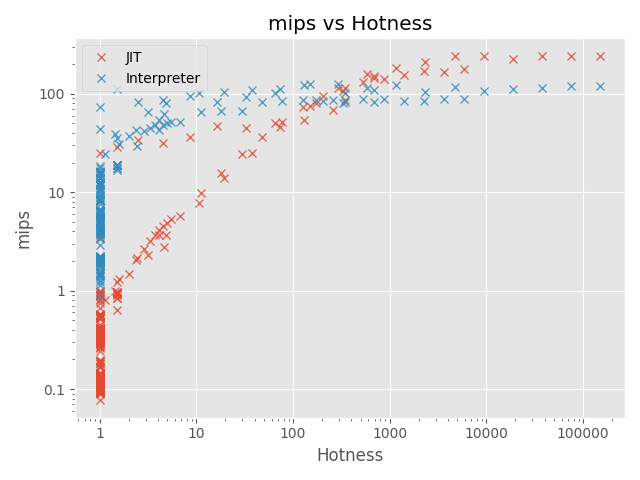
\includegraphics{output/graphs/scatter/hotness.png}
    \caption{Performance against hotness for all tests.}
    \label{figure:hotness}
\end{figure}

\subsubsection{Iteration}

\autoref{figure:primal-mips} shows the performance of the \texttt{primal(n)} test suite. It can be seen that as \texttt{n} increases, the performance increases rapidly on both SUTs.

The intepreter has higher initial performance but stabilises at a lower peak performance and at a lower value of \texttt{n}. This is because the intepreter doesn't speedup much from executing the same blocks repeatadly as there is no caching or reuse involved. It does however still see a large improvement when \texttt{n} is low because at this range the fixed overheads and initialization costs are still relatively high, and hence executing more source instructions amortizes those costs. Furthermore, repeated execution of the same instructions allow the branch predictor to become more accurate and the instruction cache warmer, both contributing to increased performance.

The JIT emulator on the other hand sees a far higher peak performance, but much worse initial performance and takes longer to achieve high performance. This is because, in addition to the higher overhead costs for the JIT emulator, each block of source code also has a high associated compilation costs. As \texttt{n} increases the same blocks are executed many times, amortizing the fixed compilation costs. This allows the JIT emulator to achieve a very high performance due to its far superior execution performance.

\begin{figure}
    \centering
    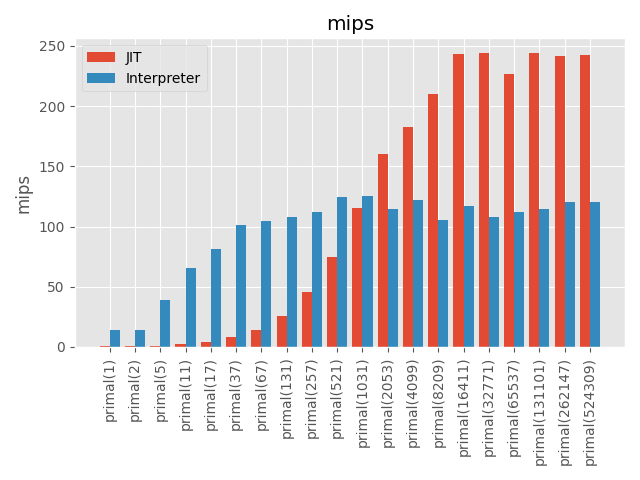
\includegraphics{output/graphs/tests/primal/mips.png}
    \caption{Performance in mips of the primal test suite.}
    \label{figure:primal-mips}
\end{figure}

\subsubsection{Recursion}

\autoref{figure:fibonacci-mips} shows the performance of the \texttt{fibonacci(n)} test suite. It has a very similar performance characteristic to the \texttt{primal(n)} test suite with some notable differences.

The overall performance for both SUTs is significantly lower. This is due to the memory instructions required for pushing and popping the stack, which have much lower emulation performance compared to arithmetic instructions.

The JIT emulator takes significantly longer to reach peak performance whereas the interpreter does not. This is because the intepreters fixed costs, such as initialization, do not change with the program being executed. The JIT emulator on the other hand has additional costs for every block that needs compiling, and the \texttt{fibonacci(n)} program contains more source blocks. This means there is a larger initial cost which takes longer to amortize.

\begin{figure}
    \centering
    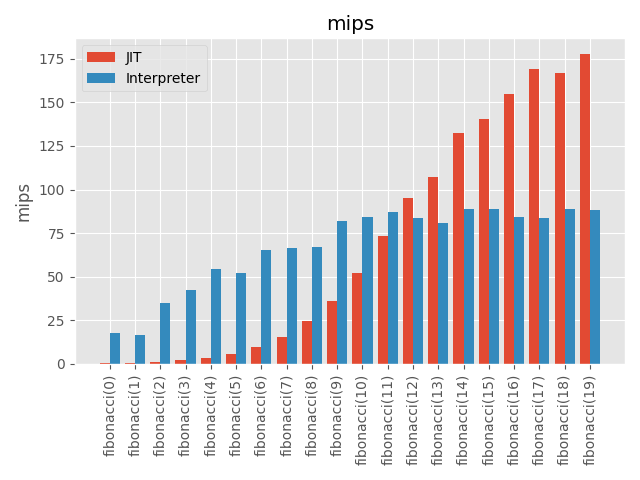
\includegraphics{output/graphs/tests/fibonacci/mips.png}
    \caption{Performance in mips of the fibonacci test suite.}
    \label{figure:fibonacci-mips}
\end{figure}

\subsubsection{Memory Intensive}
